\documentclass[aspectratio=169,10pt]{beamer}
\usetheme{Madrid}
\usepackage[T1]{fontenc}

\usepackage{fancybox,graphicx,hyperref,url}
\usepackage{tikz}
\usetikzlibrary{shapes,arrows}
\usetikzlibrary{positioning}
\usepackage{booktabs}
\usepackage{enumitem}

\usepackage{listings}
\usepackage{pdfpages}
\usepackage{lstautogobble}

\usepackage[listings,skins,breakable,xparse]{tcolorbox}
\tcbuselibrary{theorems}
\tcbset{highlight math/.append style={boxrule=0pt,
                                      frame hidden,
                                      colback=yellow!40!white,
                                      sharp corners}}

\usepackage{xpatch}
\usepackage{xcolor}
\usepackage{realboxes}
\usetikzlibrary{fit}
\usetikzlibrary{shadings}
\usetikzlibrary{shapes.arrows,shadows.blur}

\pgfdeclarefunctionalshading{Hermite-Gaussian modes}{\pgfpoint{-25bp}{-25bp}}{\pgfpoint{25bp}{25bp}}{}{
    10 atan sin 1000 mul cos 1 add
    exch
    10 atan sin 1000 mul cos 1 add
    mul 4 div
    dup dup
}

\makeatletter
\xpretocmd\lstinline{\Colorbox{yellow!10!white}\bgroup\appto\lst@DeInit{\egroup}}{}{}
\makeatother

\definecolor{my_red}{RGB}{128, 0, 0}

\lstset{captionpos=b}
\lstset{numberbychapter=false}
\lstset{autogobble}
% \lstset{breaklines=true}

\usepackage{tikz}
\usepackage{subcaption}
\usetikzlibrary{calc, chains, decorations.pathmorphing}
\usetikzlibrary{shapes,arrows,backgrounds}
\usetikzlibrary{positioning,fit,shapes.geometric,shapes}

\setbeamercovered{transparent}

\setlistdepth{9}
\setlist[itemize,1]{label=$\bullet$}
\setlist[itemize,2]{label=$\bullet$}
\setlist[itemize,3]{label=$\bullet$}
\setlist[itemize,4]{label=$\bullet$}
\setlist[itemize,5]{label=$\bullet$}
\setlist[itemize,6]{label=$\bullet$}
\setlist[itemize,7]{label=$\bullet$}
\setlist[itemize,8]{label=$\bullet$}
\setlist[itemize,9]{label=$\bullet$}
\renewlist{itemize}{itemize}{9}

\setlist[enumerate,1]{label=$\arabic*.$}
\setlist[enumerate,2]{label=$\alph*.$}
\setlist[enumerate,3]{label=$\roman*.$}
\setlist[enumerate,4]{label=$\arabic*.$}
\setlist[enumerate,5]{label=$\alpha*$}
\setlist[enumerate,6]{label=$\roman*.$}
\setlist[enumerate,7]{label=$\arabic*.$}
\setlist[enumerate,8]{label=$\alph*.$}
\setlist[enumerate,9]{label=$\roman*.$}
\renewlist{enumerate}{enumerate}{9}

\AtBeginSection[]{
  \begin{frame}[noframenumbering]
    \vfill
    \centering
    \begin{beamercolorbox}[sep=8pt,center,shadow=true,rounded=true]{title}
      \usebeamerfont{title}\insertsectionhead\par%
    \end{beamercolorbox}
    \vfill
  \end{frame}
}

\title[Nondeterministic Asynchronous Dataflow in Isabelle/HOL]{Nondeterministic Asynchronous Dataflow in Isabelle/HOL}

\author[Rafael Castro, Laouen Fernet and Dmitriy Traytel]{
  Rafael Castro G. Silva, Laouen Fernet and  Dmitriy Traytel\\\medskip
  {\small \url{rasi@di.ku.dk}}}

\date{14/09/2024}

% change title (done)
% (co)datatypes -> codatatypes (done)
% while_option from HOL library (done)
% coindtive principle -> coinduction principle (done)
% remove next step slide, andd as a bullet (done)
% explain slice in more detail (done)
% mention selectors in llist slide, drop lmap, drop lset (done)
% move count operator example to slide that introduce op type (done)
% modeling lazy list processors which do not care about time (done)
% reduce Corecursion is like recursion line (done)
% why partial order? mention timely dataflow (done)
% explain what incremental, and set expectation for example (done)
% move arrows (done)
% Change push to out, done to out (done)
% put star footnote on op type saying it is simplified compare to the paper, also in the composition lemma (done)
% write the lapp lemma about lfinite (done)
% show coinduction principle for llist (done)
% add link llist afp (done)
% on produce slide, metion lshift as friend (point to freinds with benefits paper) (done)
% justify the compositional reasoning with lines of code for each building block (done)
% slide about tecnicques used, coinduction principles, friends, reasoning up to friends, generalization using skip_op, combining coinduction and induction, coinduction up to congruence for coinductive predicates, say our paper is more detailed in these topics
%
% add definition of batch_op, and all 4 properties

\institute[UCPH]{
  Department of Computer Science \\
  University of Copenhagen}

\begin{document}
\setbeamercovered{invisible}
% \setbeamercovered{dynamic}

\begin{frame}
  \titlepage

\end{frame}
\section{Introduction}

\begin{frame}[fragile]
  \frametitle{Time-Aware Stream Processing}
  \begin{itemize}
    \item What is Time-Aware Stream Processing?
          \begin{itemize}
                  \pause
            \item Stream Processing: programs that compute (possibly) unbounded sequences of data (streams)
                  \pause
            \item Time-Aware: Data has timestamp metadata; timestamps are bounded by watermarks
                  \begin{itemize}
                    \item Timestamp: A partially-ordered value associated with the data (e.g., unix-time, int, pairs of ints, etc...)
                    \item Watermark: A value of the same type of the timestamp. Represents data-completeness.
                          \begin{figure}
                            \centering
                            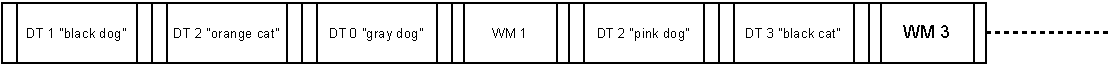
\includegraphics[width=.75\textwidth]{stream_ex1.pdf}
                          \end{figure}
                  \end{itemize}
          \end{itemize}
          \pause
    \item Asynchronous Dataflow Programming: Directed graph of interconnected operators that perform event-wise transformations
    \item E.g.: Apache Flink, Apache Samza, Apache Spark, Google Cloud Dataflow, and Timely Dataflow
          \vspace*{-1ex}
          \begin{overlayarea}{\textwidth}{.1\textheight}
            \centering
            \begin{figure}
              \centering
              \only<2->{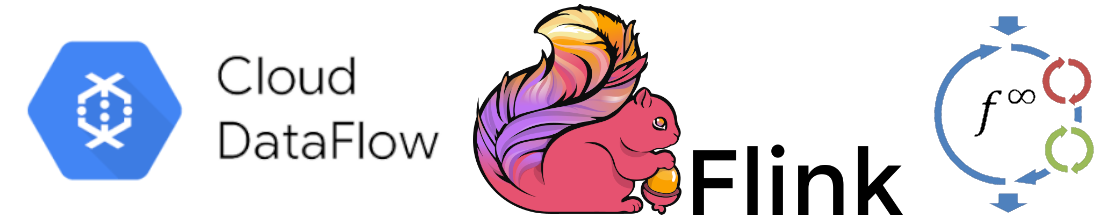
\includegraphics[scale=0.1]{all.png}}
            \end{figure}
          \end{overlayarea}
          \vspace*{-1ex}
          \pause
    \item Why?
          \begin{itemize}
            \item Highly Parallel
            \item Low latency (output as soon as possible)
            \item Incremental computing (re-uses previous computations)
          \end{itemize}
  \end{itemize}
\end{frame}


\section{Formalization in Isabelle/HOL}

\begin{frame}[fragile]
  \frametitle{Isabelle/HOL}
  \begin{itemize}
    \item Classical higher-order logic (HOL): Simple Typed Lambda Calculus + (Hilbert) axiom of choice + axiom of infinity + rank-1 polymorphism
          \pause
    \item Isabelle: A generic proof assistant
          \begin{overlayarea}{\textwidth}{.45\textheight}
            \centering
            \begin{figure}
              \centering
              \only<2>{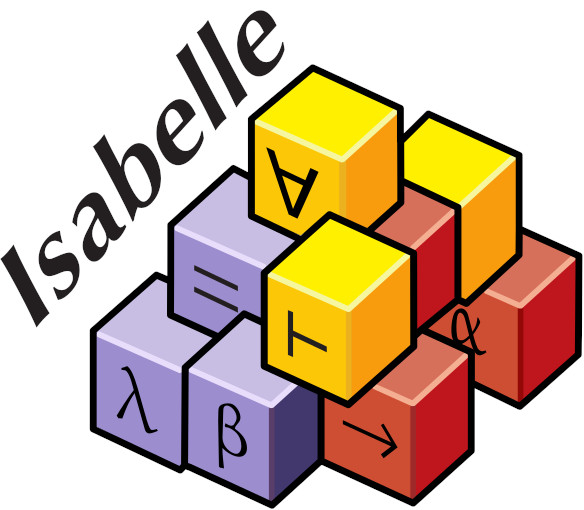
\includegraphics[scale=0.15]{isabelle}}
            \end{figure}
          \end{overlayarea}
    \item Isabelle/HOL: Isabelle's flavor of HOL
  \end{itemize}
\end{frame}

\begin{frame}[fragile]
  \frametitle{Isabelle/HOL: Codatatypes}
  \begin{itemize}
    \item Codatatypes
          \vspace*{-1ex}
  \end{itemize}
\end{frame}


% \begin{frame}[fragile,noframenumbering]
%   \frametitle{Isabelle/HOL: (Co)datatypes}
%   \begin{itemize}
%     \item Datatypes and Codatatypes
%           \vspace*{-1ex}
%           \begin{tcblisting}{hbox,listing only,listing options={language=isabelle,aboveskip=0pt,belowskip=0pt},size=fbox,boxrule=0pt,frame hidden,arc=0pt,colback=yellow!10!white}
%             codatatype (lset: 'a) llist = lnull: LNil | LCons (lhd: 'a) (ltl: "'a llist")
%             for map: lmap where "ltl LNil = LNil"
%           \end{tcblisting}
%           \vspace*{-1ex}
%     \item Examples:
%           \begin{itemize}
%             \item \is{LNil}
%             \item \is{LCons 1 (LCons 2 (LCons 3 LNil))}
%             \item \is{LCons 0 (LCons 0 (LCons 0 (...)))}
%           \end{itemize}
%           \vspace*{-1ex}
%     \item Coinductive principle for lazy list equality:
%           \begin{itemize}
%             \item Show that there is a ``pair of goggles '' (relation) that makes them to look the same:
%                   \begin{itemize}
%                     \item The first lazy list is empty iff second is
%                     \item They have the same head
%                     \item Their tail looks the same
%                   \end{itemize}
%           \end{itemize}
%   \end{itemize}
%   \vspace*{-1ex}
%   \begin{overlayarea}{\textwidth}{.45\textheight}
%     \begin{figure}
%       \centering
%       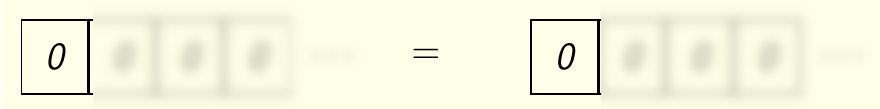
\includegraphics[scale=0.3]{equality_2.png}
%     \end{figure}
%   \end{overlayarea}
% \end{frame}

% % TODO add notes for explaining codatatype command
% \begin{frame}[fragile,noframenumbering]
%   \frametitle{Isabelle/HOL: (Co)datatypes}
%   \begin{itemize}
%     \item Datatypes and Codatatypes
%           \vspace*{-1ex}
%           \begin{tcblisting}{hbox,listing only,listing options={language=isabelle,aboveskip=0pt,belowskip=0pt},size=fbox,boxrule=0pt,frame hidden,arc=0pt,colback=yellow!10!white}
%             codatatype (lset: 'a) llist = lnull: LNil | LCons (lhd: 'a) (ltl: "'a llist")
%             for map: lmap where "ltl LNil = LNil"
%           \end{tcblisting}
%           \vspace*{-1ex}
%     \item Examples:
%           \begin{itemize}
%             \item \is{LNil}
%             \item \is{LCons 1 (LCons 2 (LCons 3 LNil))}
%             \item \is{LCons 0 (LCons 0 (LCons 0 (...)))}
%           \end{itemize}
%           \vspace*{-1ex}
%     \item Coinductive principle for lazy list equality:
%           \begin{itemize}
%             \item Show that there is a ``pair of goggles '' (relation) that makes them to look the same:
%                   \begin{itemize}
%                     \item The first lazy list is empty iff second is
%                     \item They have the same head
%                     \item Their tail looks the same
%                   \end{itemize}
%           \end{itemize}
%   \end{itemize}
%   \vspace*{-1ex}
%   \begin{overlayarea}{\textwidth}{.45\textheight}
%     \begin{figure}
%       \centering
%       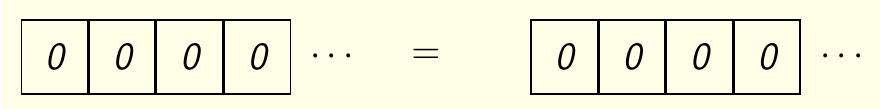
\includegraphics[scale=0.3]{equality.png}
%     \end{figure}
%   \end{overlayarea}
% \end{frame}

\begin{frame}[fragile]
  \frametitle{Isabelle/HOL: Corecursion}
  \begin{itemize}
    \item Recursion: always eventually reduces an argument
    \item Corecursion: always eventually produces something
          \pause
    \item Corec:
%           \begin{tcblisting}{hbox,listing only,listing options={language=isabelle,aboveskip=0pt,belowskip=0pt},size=fbox,boxrule=0pt,frame hidden,arc=0pt,colback=yellow!10!white}
% corec lapp :: "'a llist => 'a llist => 'a llist" where
% "lapp lxs lys = case lxs of LNil => lys | LCons x lxs' => LCons x (lapp lxs' lys)"

% \<not> lfinite lxs ==> lapp lxs lys = lxs
%           \end{tcblisting}
          % \pause
    % \item Friendly function
    %       \begin{itemize}
    %         \item Preserves productivity: it may consume at most one constructor to produce one constructor.
    %         \item \is{lshift} (\is{@@}) is proved to a be friend
    %       \end{itemize}
    %       \pause
    % \item Coinduction up to congruence: Coinduction for Lazy list equality can be extended to compare an entire finite prefix through a congruence relation
  \end{itemize}
\end{frame}

\begin{frame}[fragile]
  \frametitle{Isabelle/HOL: (Co)inductive Predicates}
  \begin{itemize}
    \item Inductive predicate
          \begin{itemize}
            \item Finite number of introduction rule applications
          \end{itemize}
%           \begin{tcblisting}{hbox,listing only,listing options={language=isabelle,aboveskip=0pt,belowskip=0pt},size=fbox,boxrule=0pt,frame hidden,arc=0pt,colback=yellow!10!white}
% inductive in_llist :: "'a => 'a llist => bool" where
%   In_llist: "in_llist x (LCons x lxs)"
% | Next_llist: "in_llist x lxs => in_llist x (LCons y lxs)"

% in_llist 2 (LCons 1 (LCons (2 (...))))
%           \end{tcblisting}
          \pause
    \item Coinductive predicate
          \begin{itemize}
            \item Infinite number of introduction rule applications
          \end{itemize}
%           \begin{tcblisting}{hbox,listing only,listing options={language=isabelle,aboveskip=0pt,belowskip=0pt},size=fbox,boxrule=0pt,frame hidden,arc=0pt,colback=yellow!10!white}
% coinductive lprefix :: "'a llist => 'a llist => bool" where
%   LNil_lprefix: "lprefix LNil lys"
% | LCons_lprefix: "lprefix lxs lys => lprefix (LCons x lxs) (LCons x lys)"

% lprefix (LCons 1 (LCons (2 (...)))) (LCons 1 (LCons (2 (...))))
%           \end{tcblisting}
          \pause
    \item Coinduction principle
    % \item But not coinduction up to congruence for free
  \end{itemize}
\end{frame}


% \begin{frame}[fragile]
%   \frametitle{Compositional Reasoning}
%   \begin{itemize}
%     \item \is{batch_op} and \is{incr_op} can be composed
%           \vspace*{-1ex}
%           \begin{tcblisting}{hbox,listing only,listing options={language=isabelle,aboveskip=0pt,belowskip=0pt},size=fbox,boxrule=0pt,frame hidden,arc=0pt,colback=yellow!10!white}
% definition "incr_batch_op buf1 buf2 = comp_op (batch_op buf1) (incr_op buf2)"
%           \end{tcblisting}
%           \vspace*{-1ex}
%     \item Soundness, completeness, and monotone and productive preservation
%   \end{itemize}
% \end{frame}

% \section{Other shapes}

% \begin{frame}[fragile]
%   \frametitle{Join Operator}
%   \begin{itemize}
%     \item Relation Join
%     \item Use the \is{sum} type in the timestamps to represent two stream as one
%     \item Partial order for the \is{sum}: lefts and rights are incomparable
%     \item Defined using \is{incr_batch_op}
%     \item Soundness, completeness, and monotone and productive preservation
%   \end{itemize}
% \end{frame}

\section{Conclusion}

\begin{frame}
  \frametitle{Conclusion}
  \begin{itemize}
    \item Isabelle/HOL has a good tool set to formalize and reason about stream processing:
          \begin{itemize}
            \item Codatatypes, coinductive predicates, corecursion with friends, reasoning up to friends (congruence),
                  \begin{itemize}
                    \item Coinduction up to congruence principle is automatically derived for codatatypes (but not for coinductive principles)
                  \end{itemize}
          \end{itemize}
    \item Next step: Feedback loop
  \end{itemize}
\end{frame}
% slide about tecnicques used, coinduction principles, friends, reasoning up to friends, generalization using skip_op, combining coinduction and induction, coinduction up to congruence for coinductive predicates, say our paper is more detailed in these topics

\section{Questions, comments and suggestions}

\end{document}
